\documentclass[UTF8]{ctexart}
\usepackage{amsmath}
\usepackage{mathtools}
\usepackage{enumitem}
\usepackage{cases}
\usepackage{geometry}
\usepackage{tikz}
\geometry{a4paper,scale=0.7}
\title{每日一题(5.1)}
\author{门宇翎、李东宸}

\begin{document}
\maketitle
\begin{itemize}
\item[\textbf{1.}]若$n$为正整数,且$2^n-1$为素数,证明:$n$也为素数.\\
{\CJKfamily{kai}(门宇翎供题)}\\
\item[\textbf{2.}]如图,两个同心圆构成的圆环被均匀分割成7份,联通中间的校园共8个区域.若要给这8个区域着色,至少要用几种颜色,才能使相邻区域染不同的颜色?\\
\begin{figure}[!htbp]
\centering
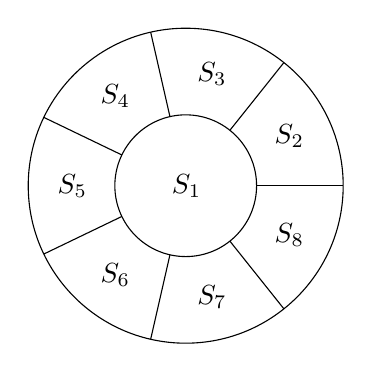
\begin{tikzpicture}
	\draw (0,0) circle(0.9);
	\node at (-0.3,0) [right]{$S_1$};
	\draw (0,0) circle(2);
	\foreach \x in {0,1,2,3,4,5,6}
		\draw [rotate={51.42857 * \x}] (0.9,0)--(2,0);
	\node at (1.0064,0.6291)[right]{$S_2$};
	\node at (0.0227,1.4136)[right]{$S_3$};
	\node at (-1.2041,1.1336)[right]{$S_4$};
	\node at (-1.75,0)[right]{$S_5$};
	\node at (-1.2041,-1.1337)[right]{$S_6$};
	\node at (0.0227,-1.4136)[right]{$S_7$};
	\node at (1.0064,-0.6291)[right]{$S_8$};

\end{tikzpicture}
\end{figure}
{\CJKfamily{kai}(李东宸供题)}\\
\end{itemize}

\end{document}